\newcommand\thC{\(\theta^1\)\,Ori~C}
\defcitealias{Canto:1996}{CRW}
\newcommand\CRW{\citetalias{Canto:1996}}


\section{Thin-shell bow shock models}
\label{sec:crw-scenario}

More physically realistic examples of bow shapes are provided by
steady-state hydrodynamic models for the interaction of hypersonic
flows in the thin-shell limit.  The classic examples are the solutions
for the wind--parallel stream and wind--wind problems (see
\S~\ref{sec:intro}) of \citet[][hereafter \CRW{}]{Canto:1996}, where
it is assumed that the two shocks are highly radiative and that the
post-shock flows are perfectly mixed to form a single shell of
negligible thickness. In this approximation, the shape of the shell is
found algebraically by \CRW{} from conservation of linear and angular
momentum, following an approach first outlined in
\citet{Wilkin:1996a}.  For the wind--stream case, the resulting bow
shape was dubbed \textit{wilkinoid} by \citet{Cox:2012a} and has the
form:
\begin{equation}
  \label{eq:wilkinoid-R-theta}
  R(\theta) = R_0\csc\theta\left( 3(1-\theta\cot\theta) \right)^{1/2} \ .
\end{equation}

For the wind--wind case, a family of solutions are found that depend on
the value of \(\beta\), the wind momentum ratio,\footnote{%
  By always placing the weaker of the two winds at the origin, it is
  only necessary to consider \(\beta \le 1\).  } %
see Figure~\ref{fig:crw-schema},
equations~(\ref{eq:stagnation-radius}, \ref{eq:beta-definition}), and
surrounding discussion in \S~\ref{sec:intro}.  We propose that these
shapes be called \textit{cantoids}.  The exact solution for the
cantoid shapes (eqs.~[23, 24] of \CRW{}) is only obtainable in
implicit form, but an approximate explicit solution (eq.~[26] of
\CRW{}) is very accurate for \(\beta \le 0.1\).  The wilkinoid shape
corresponds to the \(\beta \to 0\) limit of the cantoids.  Note that \CRW{}
employ cylindrical polar coordinates, \(z\) and \(r\), see our
Figure~\ref{fig:crw-schema}, and we follow this usage for the
thin-shell models discussed in this section.  \CRW{}'s \(z\) axis
corresponds to the cartesian \(x\) axis used in
sections~\ref{sec:projection} and \ref{sec:conic} of the current
paper, while the \(r\) axis corresponds to \(y\) when \(\phi = 0\).

A generalization of the cantoids to the case of an
anisotropic\footnote{Note that the wind anisotropy axis must be
  aligned with the star--star axis to maintain cylindrical symmetry.}
inner wind is developed next, giving rise
to what we call \textit{ancantoids}, which depend on an anisotropy
index, \(k\), in addition to \(\beta\).  

\subsection{Bow shocks from anisotropic wind--wind interactions}
\label{sec:ancantoid}
\begin{figure}
  \centering
  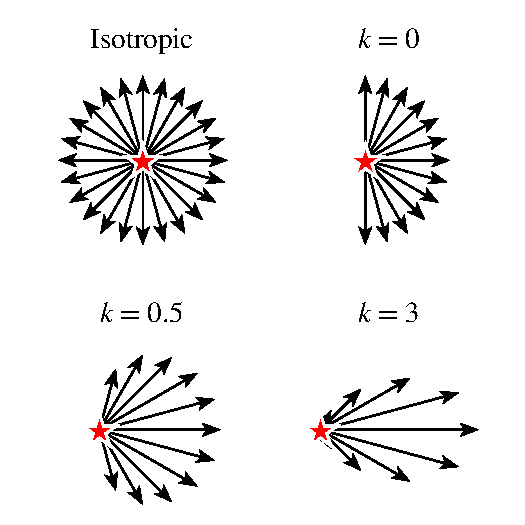
\includegraphics[width=\linewidth]{figs/anisotropic-arrows}
  \caption[]{Schematic diagram of wind flow patterns in isotropic and
    non-isotropic cases for different values of the anisotropy index,
    \(k\).  Arrow length represents the wind momentum loss rate per
    solid angle.}
  \label{fig:anisotropic-arrows}
\end{figure}


We wish to generalize the results of \citet[\CRW{}]{Canto:1996} to the
case where the inner wind is no longer isotropic, but instead has a
density that falls off with angle, \(\theta\), away from the symmetry axis.
Specifically, at some fiducial spherical radius, \(R_0\), from the
origin, the wind mass density is given by
\begin{equation}
  \label{eq:ancantoid-density}
  \rho(R_0, \theta) =
  \begin{cases}
    \rho_0 \cos^k \theta & \text{for \(\theta \le \ang{90}\)} \\
    0 & \text{for \(\theta > \ang{90}\)}
  \end{cases}
  \ ,
\end{equation}
where \(\rho_0\) is the density on the symmetry axis and \(k \ge 0\) is an
\textit{anisotropy index}.  The wind velocity is still assumed to be
constant and the wind streamlines to be radial, so the radial
variation of density at each angle is
\(\rho(R, \theta) = \rho(R_0, \theta)\, (R/R_0)^{-2}\) and the wind mass loss rate and
momentum loss rate per solid angle both have the same \(\cos^k\theta\)
dependence as the density.  Examples are shown in
Figure~\ref{fig:anisotropic-arrows} for a variety of different values
of \(k\).  As \(k\) increases, the wind becomes increasingly jet-like.

Our primary motivation for considering such an anisotropic wind is the
case of the Orion Nebula proplyds and their interaction with the
stellar wind of the massive star \thC{}
\citep{Garcia-Arredondo:2001a}.  The inner ``wind'' in this case is
the transonic photoevaporation flow away from a roughly hemispherical
ionization front, where photoionization equilibrium, together with
monodirectional illumination of the front, implies that the ionized
hydrogen density, \(n\), satisfies \(n^2 \propto \cos \theta\), which is
equivalent to \(k = 0.5\) in equation~\eqref{eq:ancantoid-density}.
Since the primary source of ionizing photons is the same star that is
the source of the outer wind, it is natural that the inner wind's axis
should be aligned with the star--star axis in this case.  For other
potential causes of wind anisotropy (for instance, bipolar flow from
an accretion disk), there is no particular reason for the axes to be
aligned, so cylindrical symmetry would be broken.  Nevertheless, we
calculate results for general \(k\) with aligned axes, so as to
provide a richer variety of cylindrically symmetric bow shock shapes
than are seen in the cantoids.

\begin{figure}
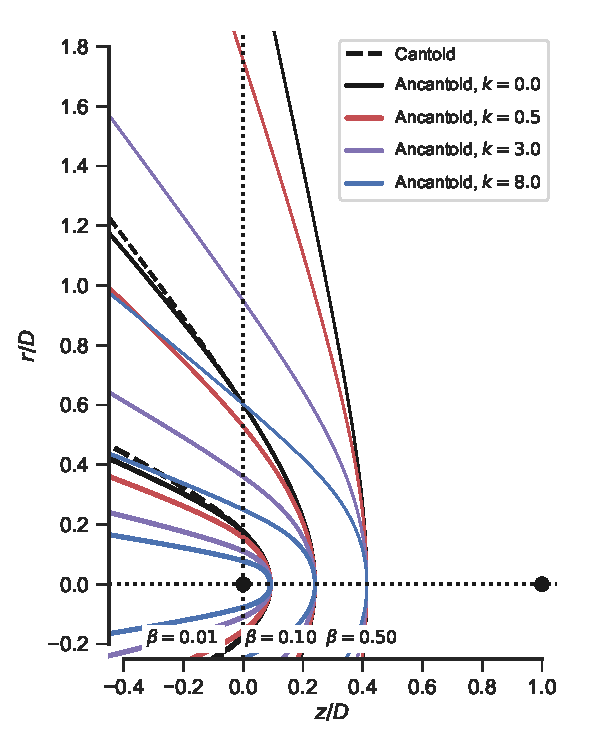
\includegraphics[width=\linewidth]{figs/ancantoid-shape}
\caption{Bow shock shapes for interacting winds in the thin-shell
  approximation: cantoids and ancantoids. Coordinates are normalized
  by $D$, the distance between the two wind sources, which are
  indicated by black dots on the axis.  The weaker source is at
  \((0.0, 0.0)\) and the stronger source is at \((1.0, 0.0)\).
  Results are shown for different values of the wind momentum ratio,
  \(\beta\) (different line widths), and for the case where the weaker
  wind is isotropic (black lines) or anisotropic (colored lines).}
\label{fig:r-beta}
\end{figure}


The general solution for the bow shock shape, \(R(\theta)\), in the \CRW{}
formalism is
\begin{equation}
  R(\theta) = \frac {\dot{J}_{\w} + \dot{J}_{\w{}1}}
  {\left(\dot{\Pi}_{\w{}r}+\dot{\Pi}_{\w{}r1}\right)\cos\theta
    - \left(\dot{\Pi}_{\w{}z}+\dot{\Pi}_{\w{}z1}\right)\sin\theta}
  \label{eq:Rmom}
\end{equation}
where \(\dot{\Pi}_{\w{}r}\), \(\dot{\Pi}_{\w{}z}\), \(\dot{J}_{\w}\) are
the accumulated linear radial momentum, linear axial momentum, and
angular momentum, respectively, due to the inner wind emitted between
the axis and \(\theta\). The equivalent quantities for the outer wind have
subscripts appended with ``1''.  The inner wind momenta for our
anisotropic case (replacing \CRW{}'s eqs.~[9, 10]) are:
\begin{gather}
  \label{eq:ancantoid-momenta}
  \begin{aligned}
    \dot{\Pi}_{\w{}z} &= \frac{k + 1}{2(k+2)}\, \dot{M}_{\w}^0 V_{\w}
    \max\left[\bigl(1- \cos^{k+2} \theta\bigr), 1 \right] \\
    \dot{\Pi}_{\w{}r} &= (k + 1)\, \dot{M}^0_{\w} V_{\w}\, I_k (\theta) 
  \end{aligned}
\end{gather}
where
\begin{equation}
  \label{eq:ancantoid-mass-loss}
  \dot{M}^0_{\w} = \frac{2 \pi} {k + 1} r_0^2 \rho_0 V_{\w}
\end{equation}
is the total mass-loss rate of the inner wind. The integral
\begin{equation}
  \label{eq:ancantoid-I-integral}
  I_k(\theta) = \int^{\max(\theta, \pi/2)}_0 \cos^k \theta \sin^2\theta \,d\theta 
\end{equation}
has an analytic solution in terms of the hypergeometric function,
\({}_2 F_1(-\tfrac12; \tfrac{1+k}2; \tfrac{3+k}2; \cos^2 \theta)\), but is
more straightforwardly calculated by numerical quadrature.  The
angular momentum of the inner wind about the origin is
\(\dot{J}_{\w} = 0\) because it is purely radial.  The outer wind
momenta are unchanged from the \CRW{} case, but are given here for
completeness:
\begin{gather}
  \label{eq:ancantoid-momenta-outer}
  \begin{aligned}
    \dot{\Pi}_{\w{}z1} & =
    -\frac{\dot{M}^0_{\w{}1}V_{\w{}1}}{4}\sin^2\theta_1\\
    \dot{\Pi}_{\w{}r1} & =
    \frac{\dot{M}^0_{\w{}1}V_{\w{}1}}{4}\left(\theta_1-\sin\theta_1\cos\theta_1\right)\\
    \dot{J}_{\w{}1} & =
    \frac{\dot{M}^0_{\w{}1}V_{\w{}1}}{4}\left(\theta_1-\sin\theta_1\cos\theta_1\right)D \ .
  \end{aligned} 
\end{gather}

\begin{figure}
  \centering
  \includegraphics[width=\linewidth]{figs/ancantoid-Pi-lambda-true}
  \caption[]{True shapes of cantoids and ancantoids in the
    \(\Pi\)--\(\Lambda\) plane, calculated according to results of
    App.~\ref{sec:thin-shell-shapes}.  For each line, \(\beta\) varies
    over the range \([0, 1]\) from lower left to upper right (although
    the black and red lines are truncated on the upper right), and
    line colors correspond to different anisotropy indices, matching
    those used in Fig.~\ref{fig:r-beta}. Circle symbols mark
    particular \(\beta\) values: \(0, 0.01, 0.1\), from largest to
    smallest circle.  Square symbols mark \(\beta = 0.5\), but with
    \(\Lambda\) calculated exactly, instead of using the approximation of
    equation~\eqref{eq:Lambda-approx}.  The white plus symbol marks
    the result for the wilkinoid:
    \((\Pi, \Lambda) = (\frac53, \sqrt{3})\).  Background shading indicates
    the domains of different quadric classes: hyperboloids (white),
    prolate spheroids (dark gray), and oblate spheroids (light gray).}
  \label{fig:ancantoid-Pi-lambda-true}
\end{figure}

We define \(\beta\) in this case as the momentum ratio \emph{on the symmetry axis}, which means that 
\begin{equation}
  \label{eq:ancantoid-momentum-ratio}
  \dot{M}^0_{\w{}1}V_{\w{}1} = 2 (k + 1)\, \beta\, \dot{M}^0_{\w} V_{\w} \ . 
\end{equation}
Substituting
equations~(\ref{eq:ancantoid-momenta}--\ref{eq:ancantoid-momentum-ratio})
into equation~\eqref{eq:Rmom} and making use of the geometric relation
between the interior angles of the triangle shown in
Figure~\ref{fig:crw-schema}:
\begin{equation}
  \label{eq:crw-angles}
  R \sin(\theta + \theta_1) = D \sin \theta_1 \ , 
\end{equation}
yields
\begin{equation}
  \label{eq:ancantoid-theta-theta1-implicit}
  \theta_1 \cot \theta_1 = 1 +
  2 \beta \left(
    I_k(\theta) \cot \theta
    - \frac{1 - \cos^{k+2} \theta} {k + 2} \right)   \ , 
\end{equation}
which is the generalization of \CRW{}'s equation~(24) to the
anisotropic case.  Equation~\eqref{eq:ancantoid-theta-theta1-implicit}
is solved numerically to give \(\theta_1(\theta)\), which is then combined with
equations~(\ref{eq:crw-angles}) and (\ref{eq:stagnation-radius}) to
give the dimensionless bow shape, \(R(\theta; \beta, k)/R_0\), where we now
explicitly indicate the dependence of the solution on two parameters:
axial momentum ratio, \(\beta\), and anisotropy index, \(k\).  We refer to
the resultant bow shapes as \textit{ancantoids}.



\begin{figure}
  \centering
  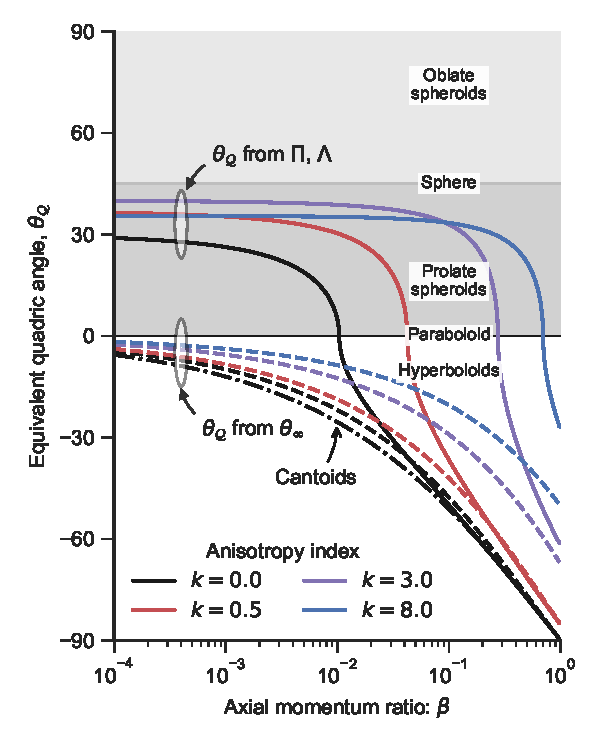
\includegraphics[width=\linewidth]{figs/ancantoid-angles}
  \caption[]{Equivalent quadric angles, \(\theta_{\Q}\), for ancantoids and
    cantoids.  Solid lines show values of \(\theta_{\Q}\) calculated from
    \((\Pi, \Lambda)\), which is representative of the shape of the head,
    while dashed lines show \(\theta_{\Q}\) calculated from
    \(\theta_\infty\), which is representative of the tail.  Dot-dashed line
    shows the result for cantoids, which differ from the \(k=0\)
    ancantoids in \(\theta_\infty\), but not in \((\Pi, \Lambda)\). Gray shading and
    line colors have the same meaning as in
    Fig.~\ref{fig:ancantoid-Pi-lambda-true}. }
  \label{fig:ancantoid-angles}
\end{figure}



\begin{figure}
  \centering
  \setkeys{Gin}{width=\linewidth}
  \begin{tabular}{@{}l@{}}
    (a) \\
    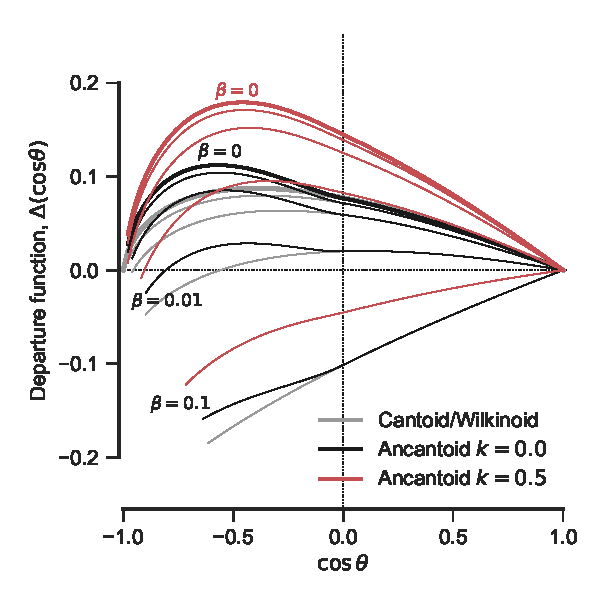
\includegraphics{figs/crw-departure} \\
    (b) \\
    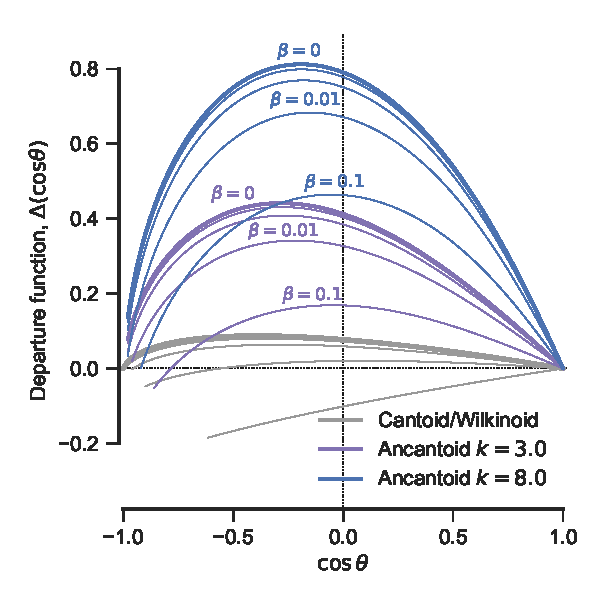
\includegraphics{figs/crw-departure-k38}
  \end{tabular}
  \caption[]{Parabolic departure function, \(\Depart(\cos\theta)\), for
    ancantoids and cantoids.  Heavy lines show the \(\beta = 0\) parallel
    stream case (Wilkinoid in the isotropic case).  Light lines show
    increasing values of \(\beta = \num{e-4}\), \num{0.001}, \num{0.01},
    \num{0.1}, as marked.  (a)~Cantoids (gray) and moderately
    anisotropic ancantoids: hemispheric, \(k = 0\) (black), and
    proplyd-like, \(k = 0.5\) (red). (b)~Cantoids (gray) and extremely
    anisotropic, jet-like ancantoids: \(k = 3\) (purple) and \(k = 8\)
    (blue).}
  \label{fig:ancantoid-departure}
\end{figure}


\begin{figure}
  \centering
  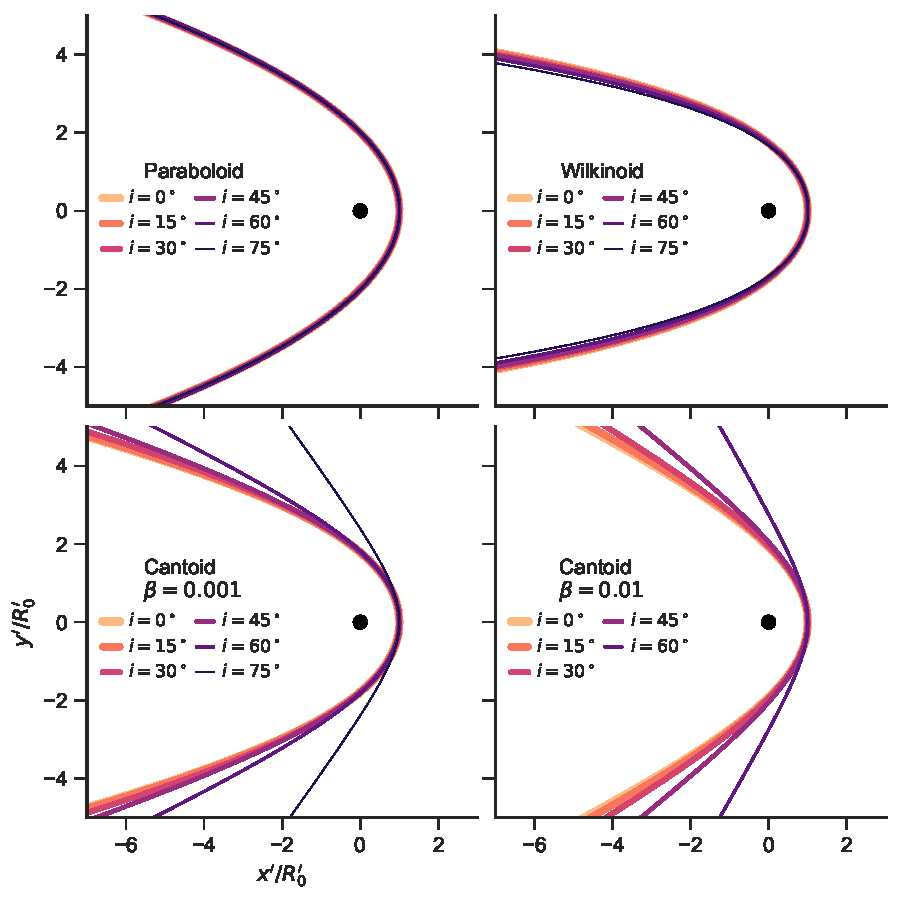
\includegraphics[width=\linewidth]{figs/test_xyprime}
  \caption{Apparent bow shapes as a function of inclination angle for
    isotropic thin shell models. (a)~Confocal paraboloid for
    comparison (shape independent of inclination).
    (b)~Wilkinoid. (c)~Cantoid, \(\beta = 0.001\). (d)~Cantoid,
    \(\beta = 0.01\). }
  \label{fig:xyprime}
\end{figure}

\begin{figure}
  \centering
  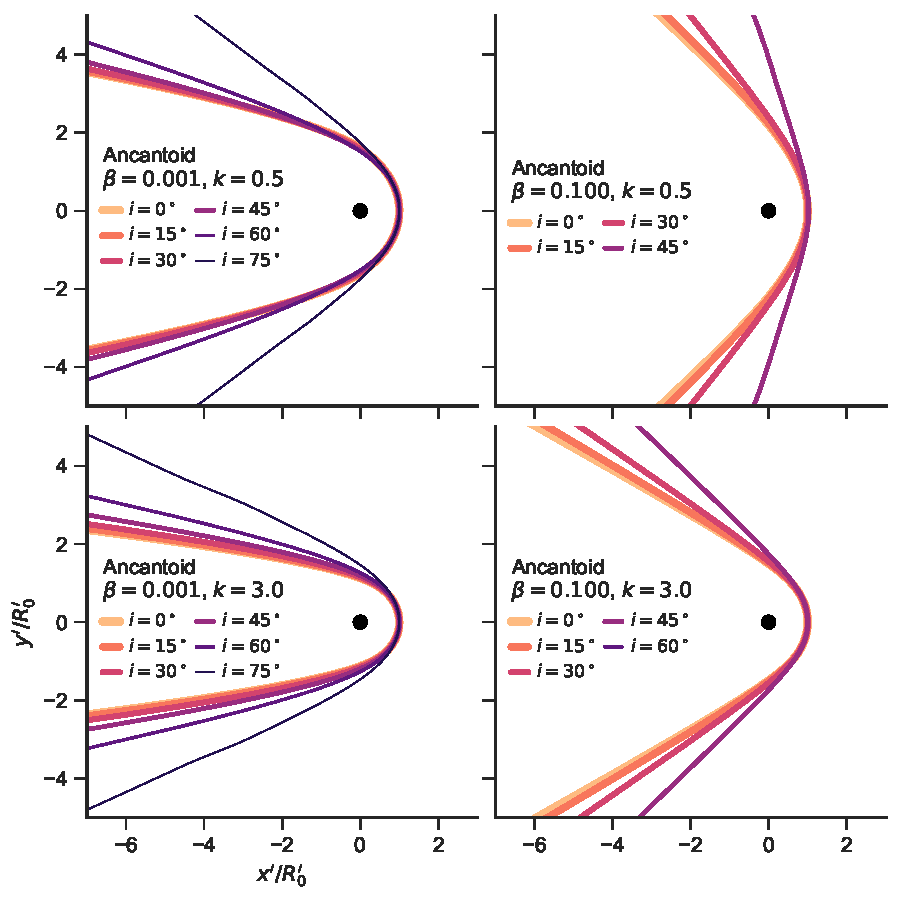
\includegraphics[width=\linewidth]{figs/test_xyprime_ancantoid}
  \caption{Further apparent bow shapes as a function of inclination
    angle for anisotropic thin shell models (ancantoids).
    (a)~\(\beta = 0.001\), \(k = 0.5\); (b) (a)~\(\beta = 0.1\),
    \(k = 0.5\); (c)~\(\beta = 0.001\) \(k = 3\); (d)
    \(\beta = 0.1\) \(k = 3\).}
  \label{fig:xyprime-ancantoid}
\end{figure}


\subsection{True shapes of cantoids and ancantoids}
\label{sec:true-cantoids-ancantoids}

The shapes of the ancantoid bow shocks are shown in
Figure~\ref{fig:r-beta} for three different values of \(\beta\), and are
compared with the \CRW{} results for cantoids (dashed curves).  The
location of these shapes in the planitude--alatude plane is shown in
Figure~\ref{fig:ancantoid-Pi-lambda-true}, where the gray background
shading indicates the zones of different quadric classes, as in
\S~\ref{sec:conic}, Figures~\ref{fig:quadric-projection-continued}
and~\ref{fig:projected-R90-Rc-snapshots}.  Values of \(\Pi\) and
\(\Lambda\) are calculated via the analytic expressions derived in
Appendix~\ref{sec:ancantoid-planitude} and
\ref{sec:ancantoid-alatude}, respectively, which are only approximate
in the case of \(\Lambda\).  However, the filled square symbols show the
exact results for \(\beta = 0.5\), which can be seen to lie extremely close
to the approximate results, even for the worst case of \(k = 0\). The
leading term in the relative error of
equation~\eqref{eq:Lambda-approx} scales as \((\beta / (k + 2))^2\), so
the approximation is even better for smaller \(\beta\) and larger \(k\).

It is apparent from Figure~\ref{fig:r-beta} that the \(k=0\) ancantoid
is identical to the cantoid for \(\theta \le \ang{90}\) (\(z > 0\), to the right
of vertical dotted line in Fig.~\ref{fig:r-beta}), but is slightly
more swept back in the far wings.\footnote{%
  \label{fn:discontinuity}
  Due to the discontinuity in the inner wind density at
  \(\theta = \ang{90}\) (see Fig.~\ref{fig:anisotropic-arrows}), there is a
  discontinuity in the second derivative of the bow shape.} %
Since the true planitude and alatude depend on \(R(\theta)\) only in the
range \(\theta = [0, \ang{90}]\), the cantoid and the \(k = 0\) ancantoid
behave identically in Figure~\ref{fig:ancantoid-Pi-lambda-true}.
There is a general tendency for the bows to be flatter and more open
with increasing \(\beta\) and decreasing \(k\), with the cantoid being
most open at a given \(\beta\).  All the models cluster close to the
diagonal \(\Lambda \simeq \Pi\) in the planitude--alatude plane, but with a tendency
for \(\Lambda > \Pi\) at higher anisotropy.  There is therefore a degeneracy
between \(\beta\) and \(k\) for higher values of \(\beta\).  The wilkinoid
shape, which corresponds to the \(\beta \to 0\) limit of the cantoids, is
marked by a white plus symbol in
Figure~\ref{fig:ancantoid-Pi-lambda-true}, and lies in the prolate
spheroid region of the plane.  Cantoids lie either in the prolate
spheroid or hyperboloid regions, according to whether \(\beta\) is less
than or greater than about \(0.01\).  For ancantoids of increasing
\(k\), this dividing point moves to higher values of \(\beta\), until
almost the entire range of models with \(k = 8\) are within the
prolate spheroid zone.

However, the true planitude and alatude, which are what would be
observed for a side-on viewing angle (\(i = 0\)), are not at all
sensitive to the behavior of the far wings of the bow shock, which has
a rather different implication as to which variety of quadric best
approximates each shape.  We illustrate this is
Figure~\ref{fig:ancantoid-angles}, which shows two different ways of
estimating the quadric angle, \(\theta_{\Q}\) (see \S~\ref{sec:conic}).
The first is from \((\Pi, \Lambda)\), as in
Figure~\ref{fig:ancantoid-Pi-lambda-true}:
\newcommand\head{^{\text{head}}}
\newcommand\tail{^{\text{tail}}}
\begin{equation}
  \label{eq:thetaQ-head}
  \theta_{\Q}\head =
  \sgn{\bigl(2 \Pi - \Lambda^2\bigr)} \;
  \tan^{-1} \Abs{2\Pi - \Lambda^2}^{1/2} \ ,
\end{equation}
which follows from equations~\eqref{eq:Tq}, \eqref{eq:thetaQ}, and
\eqref{eq:Tq-from-Pi-Lambda}.  The second is from the asymptotic
opening angle of the wings, \(\theta_\infty\) (Fig.~\ref{fig:characteristic-radii}):
\begin{equation}
  \label{eq:thetaQ-tail}
  \theta_{\Q}\tail = \theta_\infty - \ang{180} \ , 
\end{equation}
where \(\theta_\infty\) is calculated from
equation~\eqref{eq:ancantoid-theta-inf} for ancantoids, or
\eqref{eq:cantoid-theta-inf} for cantoids.  If the bow shock shape
were truly a quadric, then these two definitions would agree.
However, as seen in Figure~\ref{fig:ancantoid-angles}, this is not the
case for the cantoids and ancantoids.  While
\(\smash[b]{\theta_{\Q}\head}\) generally corresponds to a prolate spheroid
(except for the largest values of \(\beta\)),
\(\smash[b]{\theta_{\Q}\tail}\) always corresponds to a hyperbola.  This
tension between the shape of the head and the shape of the far wings
has important implications for the projected shapes (as we will see in
the next section), since the far wings influence the projected
planitude and alatude when the inclination is large.

Figure~\ref{fig:ancantoid-departure} shows the parabolic departure
function (see \S~\ref{sec:parab-depart-funct}) for the thin-shell
models. This provides an alternative perspective on the resultant bow
shapes, with two different types of behavior being apparent.  Models
with high \(\beta\) and low anisotropy behave similarly to the
hyperboloids, such as the
\((\Pi, \Lambda) = (\nicefrac32, \nicefrac83)\), \((2, \nicefrac83)\),
\((\nicefrac83, \nicefrac83)\), and \((\nicefrac32, 2)\) cases from
Figure~\ref{fig:conic-departure}.  This is the case for the
\(\beta \ge 0.01\) models in Figure~\ref{fig:ancantoid-departure}a, which
all show departure functions that become negative in the far wings
(more open than parabola) and terminate at a
\(\theta_\infty < \ang{180}\).  The second type of behavior is shown by models with
low \(\beta\) or high anisotropy, which behave like spheroids for positive
and mildly negative values of \(\cos \theta\), but, unlike the spheroids,
all tend towards \(\Depart = 0\) in the far tail as \(\cos\theta \to -1\).


% \subsection{Characteristic Radii}
% $R_0$ is obtained directly from equation (27) of \CRW{} as the distance from the inner source where the RAM pressure of the interacting winds is in equilibrium.
% %Here goes a little introduction
% For the rest of the radii we need a relation between $\theta$ and $\theta_1$ as follows:


% \begin{align}
% \theta_1\cot\theta_1 -1 = 2\beta I_k(\theta) \cot\theta - \frac{2\beta}{k+2}\left(1-\cos^{k+2}\theta\right)
% \label{eq:th1th}
% \end{align}

% Equation (\ref{eq:th1th}) is reduced to equation (24) of \CRW{} when $k=0$.
% We can obtain $R_{90}$ by following the process shown in appendix \ref{app:r90-analytic},
% which lead us to a solution for $B \equiv \frac{R_{90}}{R_0}$:

% \begin{align}
% \tilde{R}_{90} = \frac{\sqrt(3\xi)\left(1+\beta^{1/2}\right)}{(1-\xi\beta)\left(1+\frac{1}{5}\xi\beta\right)^{1/2}}
% \label{eq:B}
% \end{align}

% Now, the solution for $R_c$ is explained in appendix \ref{app:rc-analytic},
% which lead us to derive the radius of curvature at the symmetry axis:

% \begin{align}
% R_c &= R_0\left(1-2\gamma\right)^{-1} \label{eq:Rcurv} \\
% \mathrm{where:~} & \gamma = \frac{C_{k\beta}}{1+\beta^{1/2}}+\frac{1}{6}(1-2\beta^{1/2})
% \end{align}

% Finally, using equations (\ref{eq:Rcurv}) and (\ref{eq:B}) we can estimate the parameter of
% conic curves $\theta_c$ as a function of $(\beta,\xi)$ using equation (\ref{eq:Thc})

% \begin{align}
% \tan^2\theta_c &= \left| \frac{3\xi\left(1+\beta^{1/2}\right)^2}{\left(1-\xi\beta\right)^2\left(1+\frac{1}{5}\xi\beta\right)}-\frac{2}{\left(1-2\gamma\right)}\right| 
% \label{eq:thc-CRW}
% \end{align}

% \begin{figure}
% \begin{tabular}{c}
% 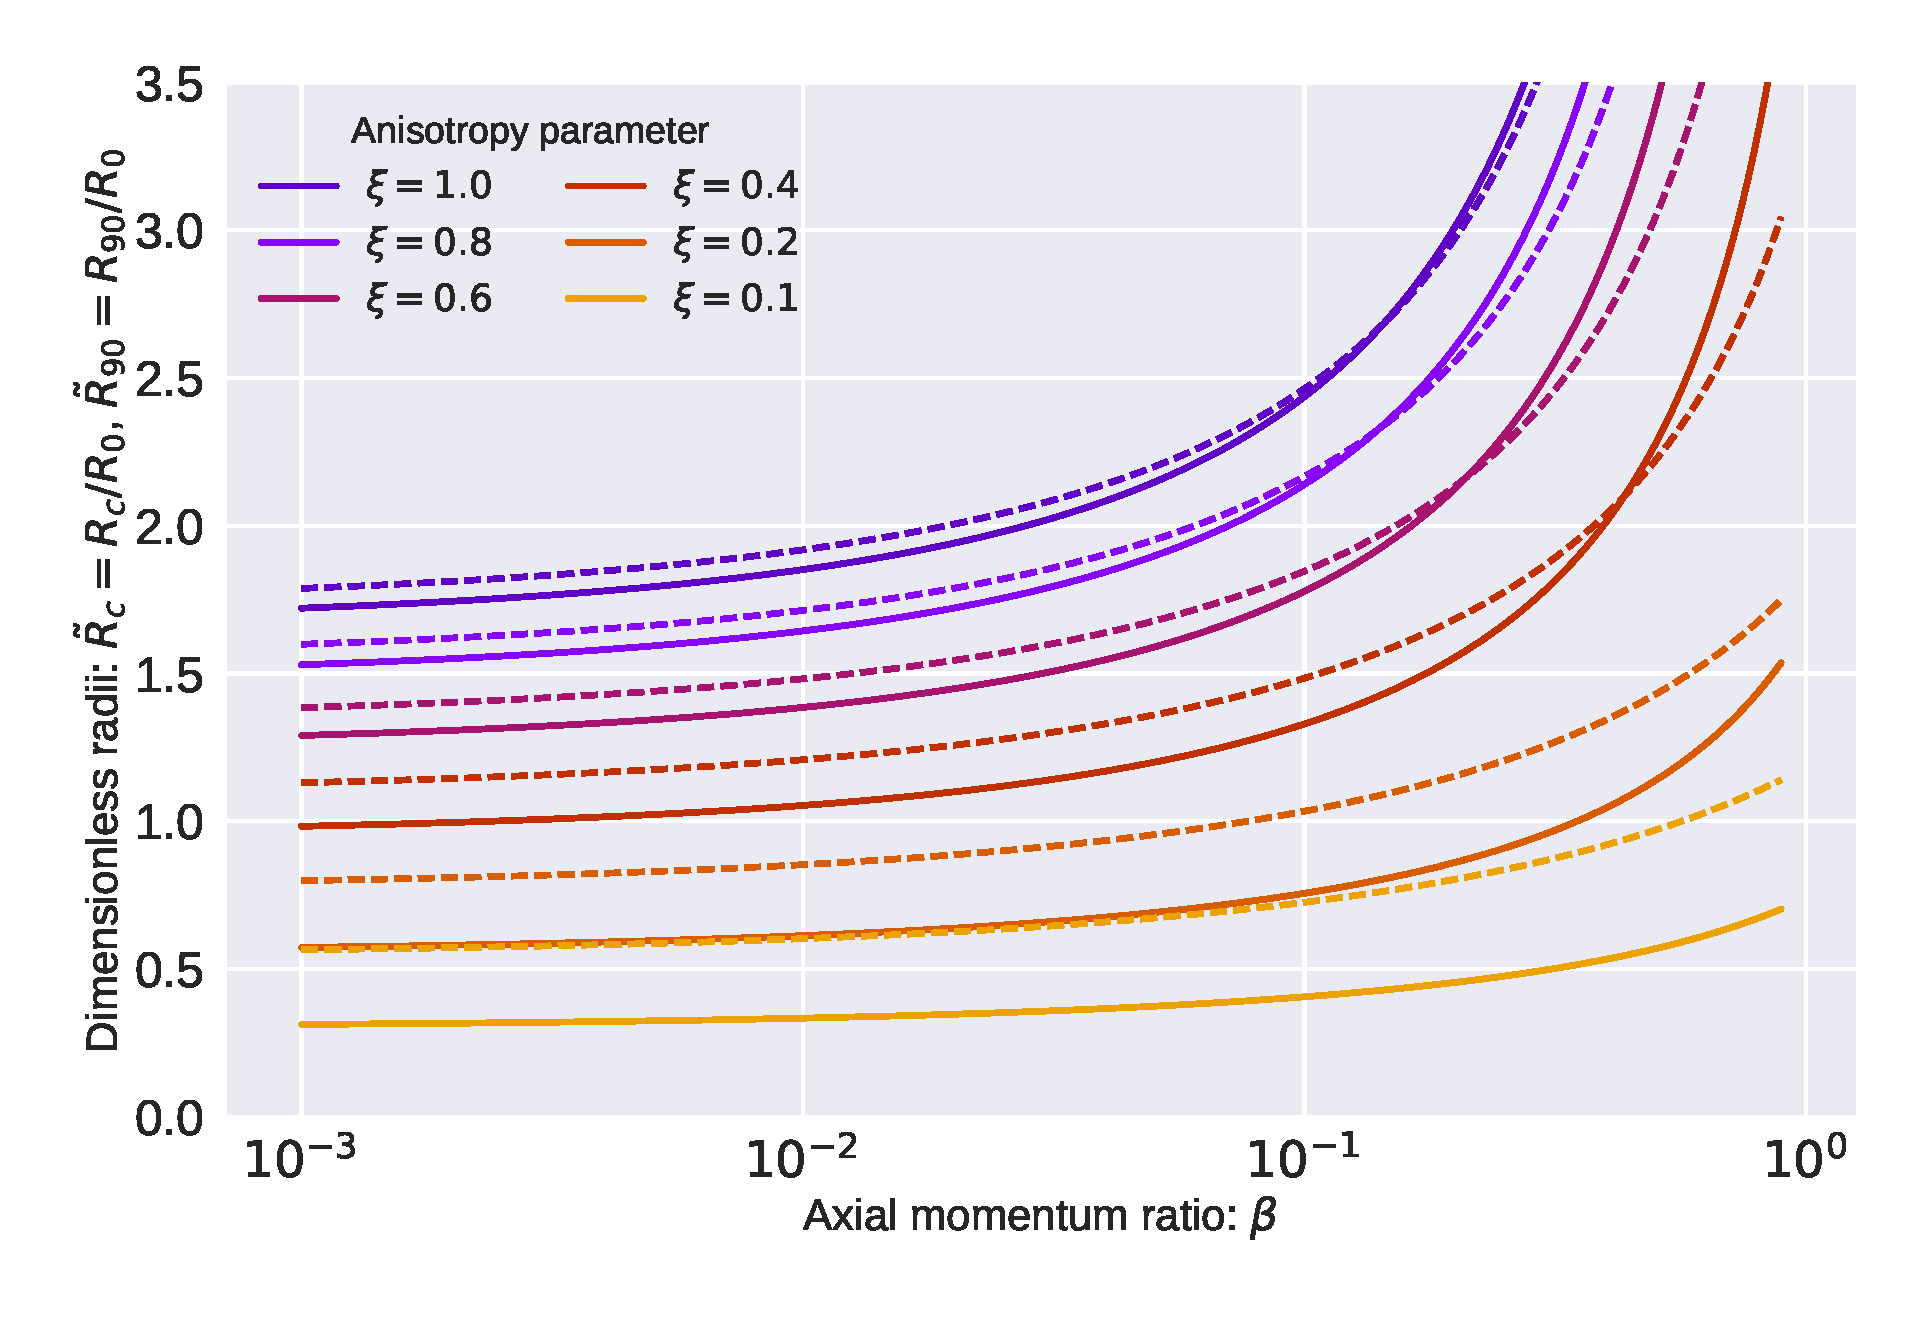
\includegraphics[width=\linewidth]{figs/AB-beta-log} \\
% 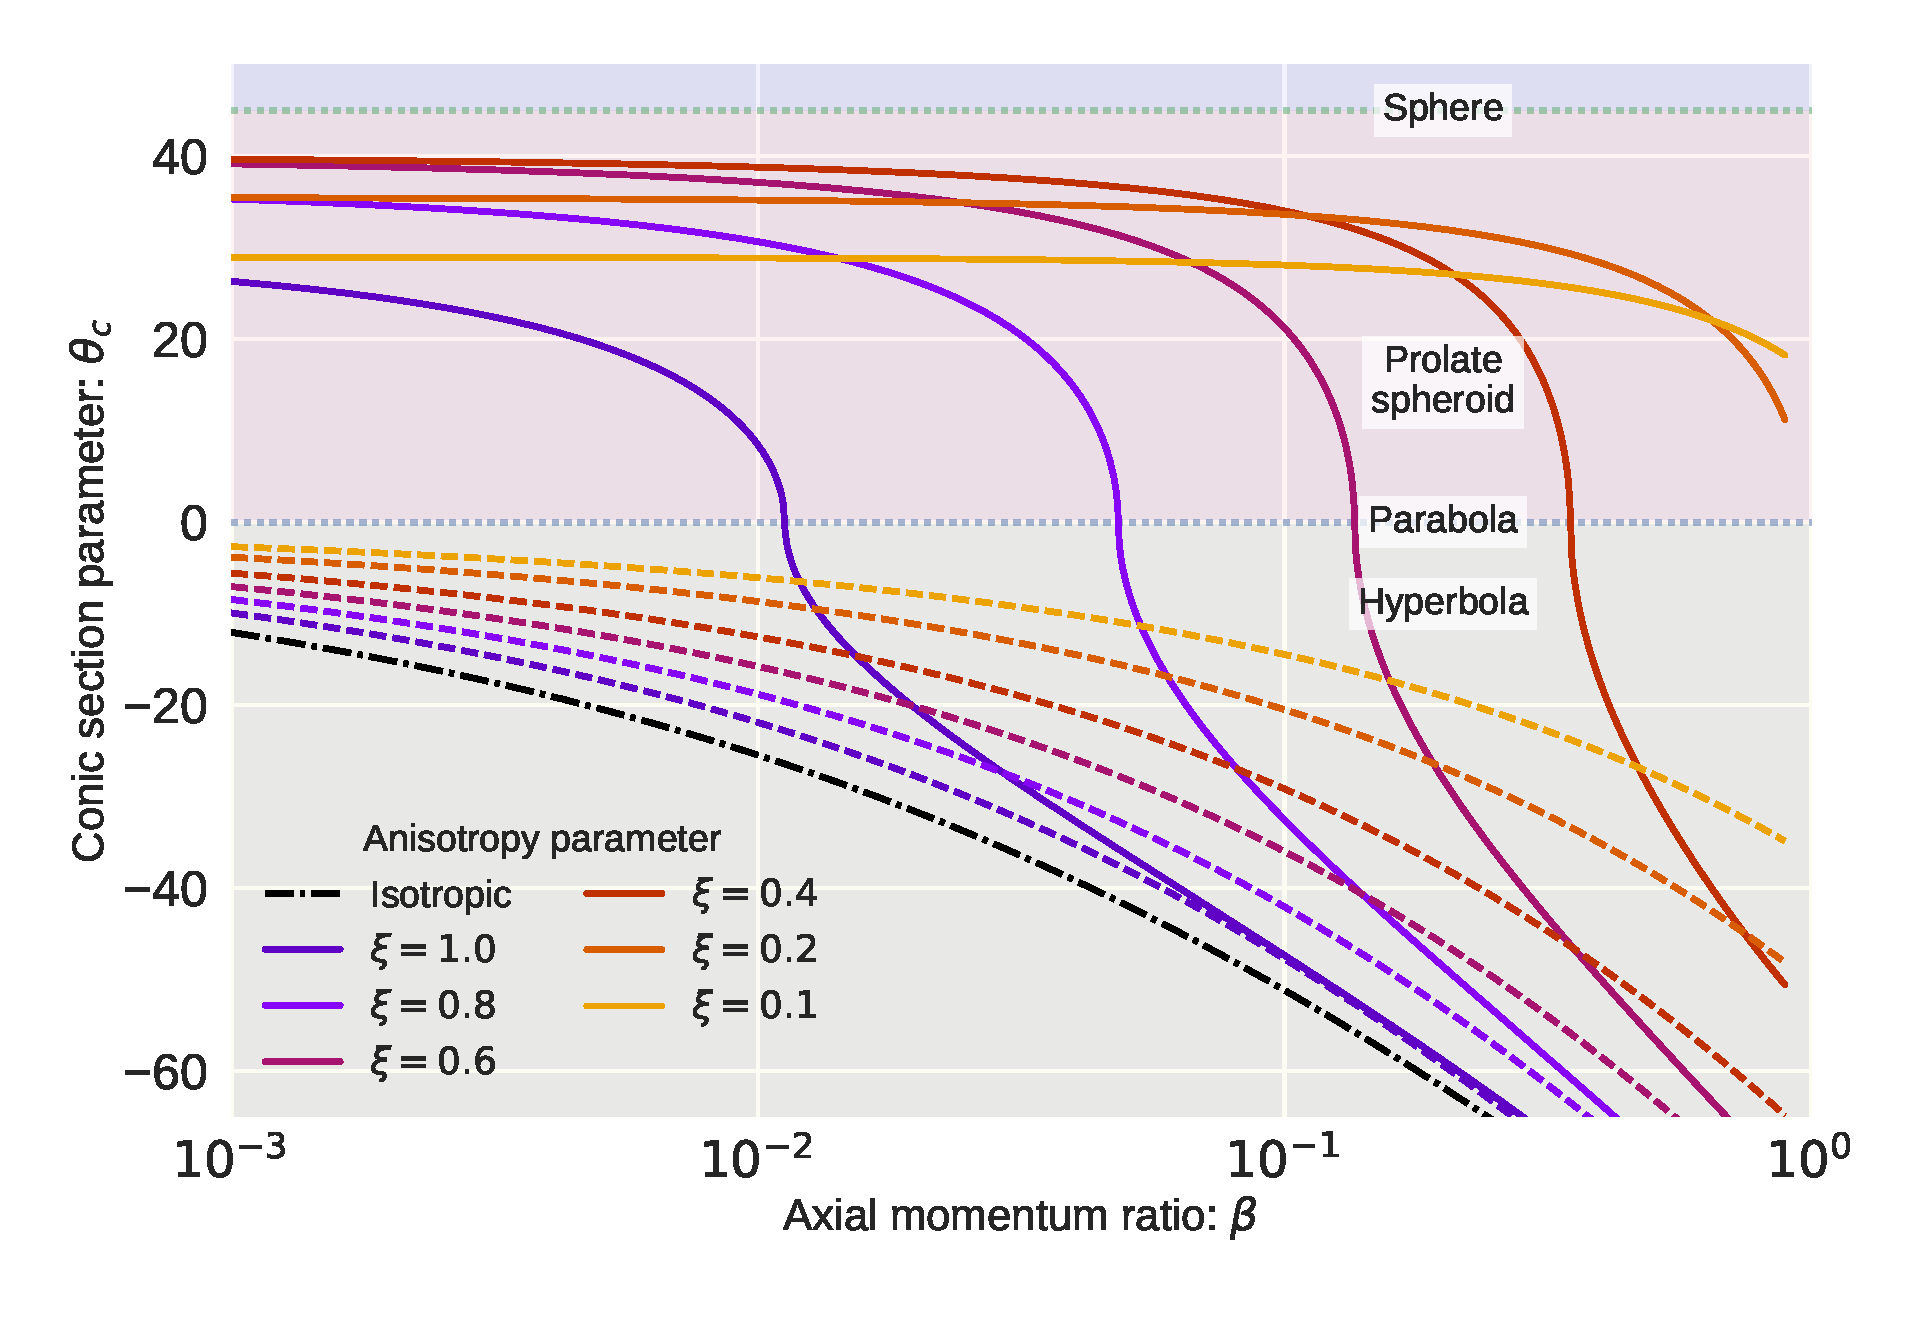
\includegraphics[width=\linewidth]{figs/thc-beta-log}
% \end{tabular}
% \caption{Top: Characteristic radii, $\tilde{R}_c = R_c/R_0$ (solid lines) and $\tilde{R}_{90}
%   = R_{90}/R_0$ (dashed lines)
%   vs $\beta$, calculated from quadric fits to the generalized CRW
%   solutions with varying degrees of isotropy $\xi$.  Bottom: Conic
%   angle $\theta_c$ vs $\beta$ for the bow 
%   shock head (solid lines) and the bow shock tail (dashed lines).}
% \label{fig:rad-beta}
% \end{figure}


% % Observationally, we can measure the projected radii. In order to estimate the model parameters is neccesary to measure at least two of the mentioned radii,
% %being $R_0$ the
% %easiest to measure. Therefore, we may compare both $R_c$ and $R_{90}$ against $R_0$ as shown in figure (\ref{fig:prop-shell-rad}). 

% With this we can use the results of section \ref{sec:conic} to estimate the projected conic shapes for bow shocks with different winds 
% momenta and different density distributions. Figure \ref{fig:rad-beta} shows equations ( \ref{eq:B}), (\ref{eq:Rcurv}) and (\ref{eq:thc-CRW}) for different anisotropy indexes. 

% \subsection{Special Case: Isotropic Wind/Parallel Flow Interaction Problem}

% This problem has already been solved in \citet{Wilkin:1996a} and \CRW{}, which have an explicit form for the shell shape, given by:

% \begin{align}
%   R(\theta) = R_0\csc\theta\left[3(1-\theta\cot\theta)\right]^{1/2} \label{eq:R-Wilkin}
% \end{align}
% Where:
% \begin{align}
%   R_0 = \left(\frac{\dot{M}_wv_w}{4\pi\rho_a v_a^2}\right)^{1/2}
% \end{align}
% And $\rho_a$ and $v_a$ being the density and the velocity of the Parallel wind, respectively.
% The characteristic radii are given by:
% \begin{align}
%   \tilde{R}_{90} &= \sqrt{3} \\
%   \tilde{R}_c &= \frac{5}{3}
% \end{align}
% The derivation of these values is developed in appendix \ref{app:ch-rad-Wilkin}

% \subsection{Fits to the tail}
% \label{sec:fits-tail}

% In most cases, the quadric fit to the head of the bowshock does a very poor job of representing the ``wings'' or ``tail''.  The bowshock tail in all cases is asymptotically hyperbolic, with 

% We therefore 
% We carry out three-level nested fits to determine the 

% For the hyperbola ``center''
% \begin{multline}
%   \label{eq:tail-analytic-x0}
%   x_{0,\mathrm{t}} = 0.7 \beta^{-0.55} \biggl[
%     C_3 \bigl(\log_{10}\beta\bigr)^3 + C_2 \bigl(\log_{10}\beta\bigr)^2 
%   \\ + C_1 \log_{10}\beta + C_0
%   \biggr]
% \end{multline}
% \begin{equation}
%   \label{eq:tail-analytic-x0-minus-a}
%   (x_{0,\mathrm{t}} - a_{\mathrm{t}}) = D_2 (\log_{10}\beta)^2 + D_1 \log_{10}\beta + D_0
% \end{equation}
% where
% \begin{alignat}{2}
%   \label{eq:tail-analytic-coeffs-c}
%   C_k &= c_{2,k} \xi^2 + c_{1,k} \xi + c_{0,k} &\quad \text{for\ } k &= \{0, 1, 2, 3\} \\
%   \label{eq:tail-analytic-coeffs-d}
%   D_k &= d_{2,k} \xi^2 + d_{1,k} \xi + d_{0,k} &\quad \text{for\ } k &= \{0, 1, 2\}
% \end{alignat}


% % \newcommand\iso{\ensuremath{^{\mathrm{iso}}}}

% % \begin{table}
% %   \caption{Coefficients for hyperbola fit to bowshock tails}
% %   \label{tab:tail-fit-coeffs}
% %   \renewcommand\arraystretch{1.2}
% %   \setlength\tabcolsep{0.5\tabcolsep}
% %   \begin{tabular}{@{}llll@{}}
% %     \toprule
% %     Equation~(\ref{eq:tail-analytic-x0}) & 
% %     \multicolumn{3}{l}{
% %     Equation~(\ref{eq:tail-analytic-coeffs-c}) \dotfill
% %     } \\ \midrule
% %     \( C\iso_0 = +1.3195     \)    
% %     & \( c_{0,0} = +2.0758   \)  
% %     & \( c_{1,0} = -0.2309   \)  
% %     & \( c_{2,0} = -0.2532   \)\\
% %       \( C\iso_1 = +0.4229     \)    
% %     & \( c_{0,1} = +0.9571   \)  
% %     & \( c_{1,1} = -0.1530   \)  
% %     & \( c_{2,1} = -0.2487   \)\\
% %       \( C\iso_2 = +0.1092     \)    
% %     & \( c_{0,2} = +0.2528   \)  
% %     & \( c_{1,2} = -0.0360   \)  
% %     & \( c_{2,2} = -0.0794   \)\\
% %       \( C\iso_3 = +0.0051     \)    
% %     & \( c_{0,3} = +0.0171   \)  
% %     & \( c_{1,3} = -0.0010   \)  
% %     & \( c_{2,3} = -0.0095   \)\\ \midrule
% %     Equation~(\ref{eq:tail-analytic-x0-minus-a}) &
% %     \multicolumn{3}{l}{
% %     Equation~(\ref{eq:tail-analytic-coeffs-d}) \dotfill
% %     } \\ \midrule
% %     \( D\iso_0 = +0.7962   \)    
% %     & \( d_{0,0} = +0.8516 \)  
% %     & \( d_{1,0} = -0.0907 \)  
% %     & \( d_{2,0} = -0.2002 \)\\
% %       \( D\iso_1 = -0.2363   \)    
% %     & \( d_{0,1} = -0.7620 \)  
% %     & \( d_{1,1} = +0.1411 \)  
% %     & \( d_{2,1} = -0.0295 \)\\
% %       \( D\iso_2 = -0.0126   \)    
% %     & \( d_{0,2} = -0.0683 \)  
% %     & \( d_{1,2} = +0.0390 \)  
% %     & \( d_{2,2} = -0.0236 \)\\
% %     \bottomrule
% %   \end{tabular}
% % \end{table}




% % \begin{figure*}
% %   \centering
% %   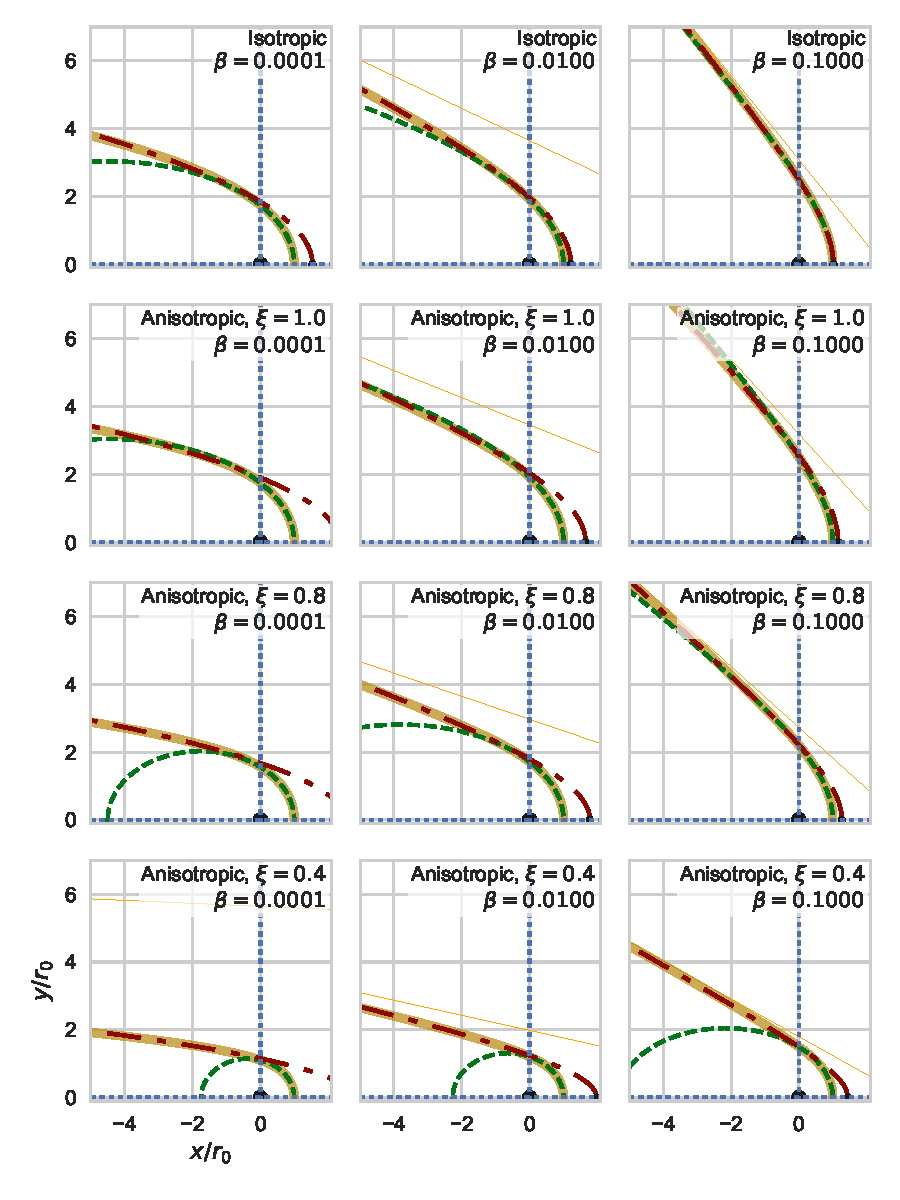
\includegraphics[width=0.8\textwidth]{figs/conic-head-tail-analytic}
% %   \caption{Double quadric fits to thin shell
% %     solutions.}
% %   \label{fig:head-tail}
% % \end{figure*}

% % \begin{figure}
% %   \centering
% %   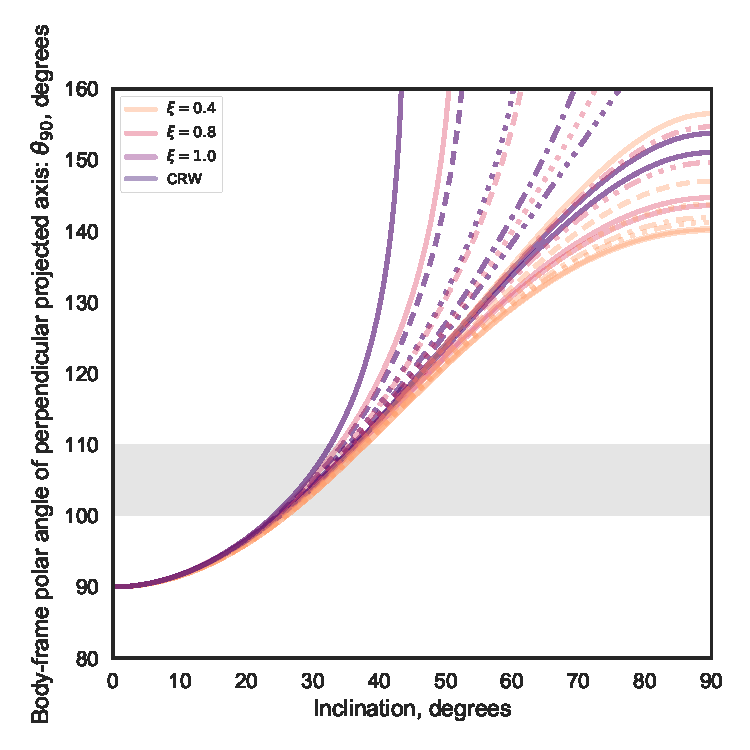
\includegraphics[width=\linewidth]{figs/two-quadric-th90-vs-i}
% %   \caption{Variation with inclination of the body-frame polar angle
% %     \(\theta_{90}\) that corresponds to the projected perpendicular radius
% %     \(R’_{90}\).  Line colors and thicknesses represent different
% %     quadrics of revolution, as in
% %     Fig.~\ref{fig:projected-R90-Rc-snapshots}.  This quantity is
% %     important because the quadric fits to the bow shock shape must be
% %     accurate for \(\theta < \theta_{90}\) in order to give a reliable estimate
% %     for \(R’_{90}\).}
% %   \label{fig:projected-th90}
% % \end{figure}



% \begin{figure*}
%   \centering
%   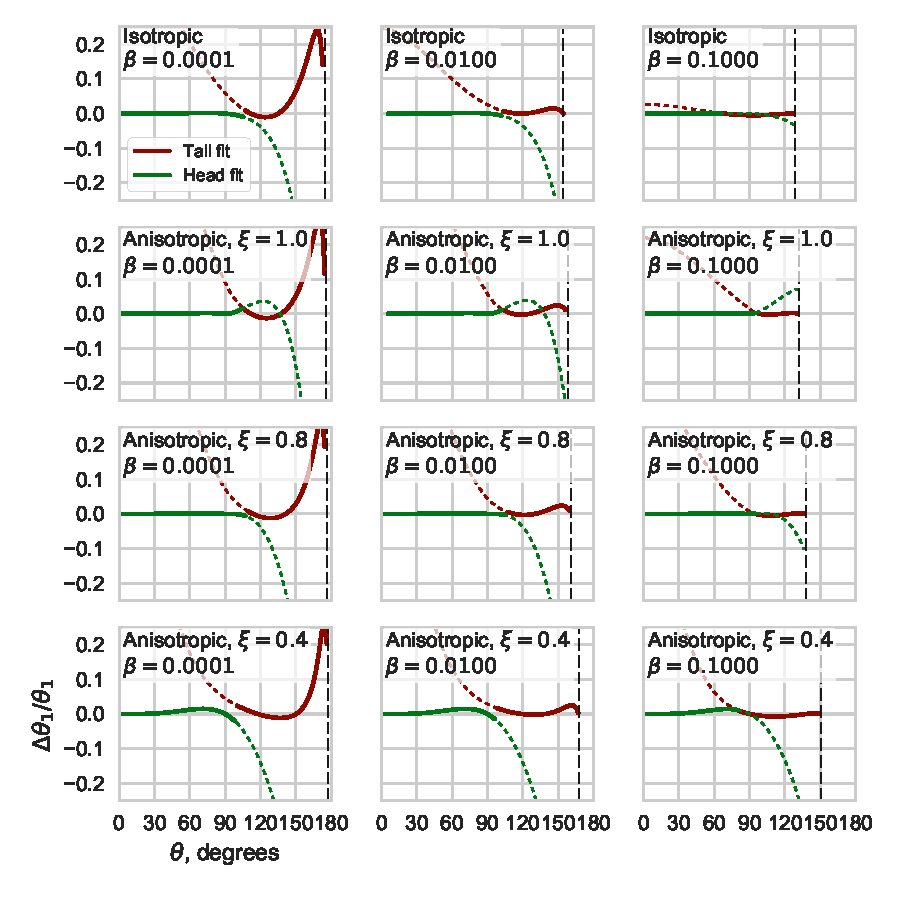
\includegraphics[width=0.8\textwidth]{figs/conic-head-tail-residuals}
%   \caption[]{Residuals of double quadric fits to thin shell solutions.
%     Residuals are expressed as the fractional error in the
%     complementary angle \(\theta_1\) (see Fig.~\ref{fig:crw-schema}) for
%     the same parameters as are shown in Fig.~\ref{fig:head-tail}.}
%   \label{fig:head-tail-residuals}
% \end{figure*}

% \subsection{Projection effects in the thin shell model}
% \label{sec:proj-effects-thin}


\begin{figure}
  \centering
  \setkeys{Gin}{width=\linewidth}
  \begin{tabular}{@{}l@{}}
    (a) \\
    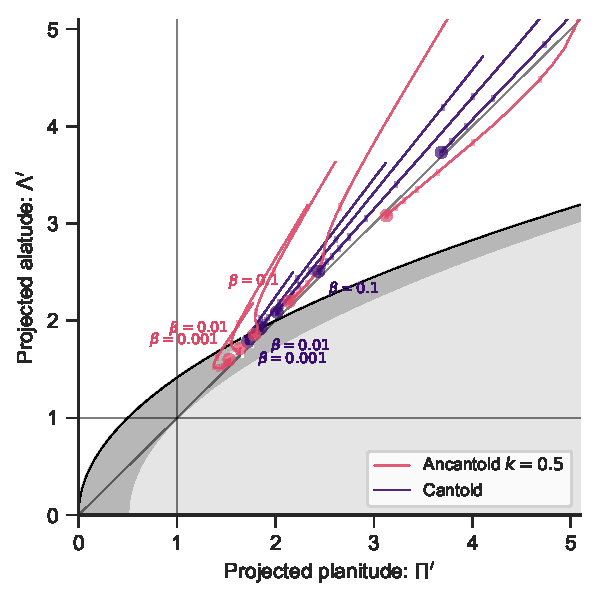
\includegraphics{figs/ancantoid-R90-vs-Rc-a} \\
    (b) \\
    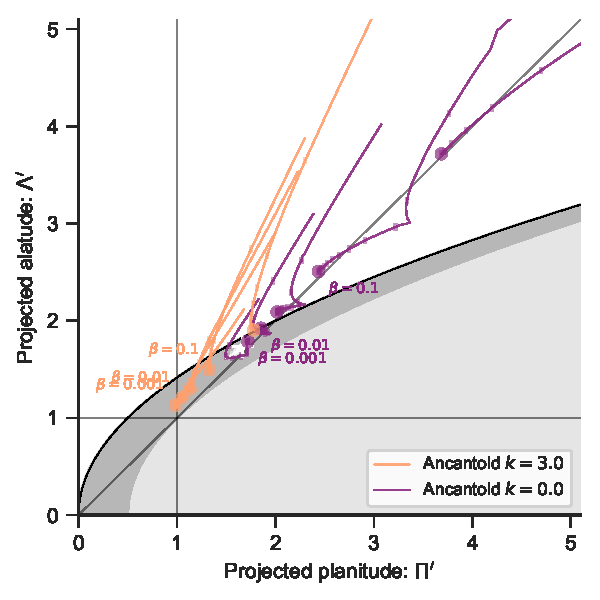
\includegraphics{figs/ancantoid-R90-vs-Rc-b}
  \end{tabular}
  \caption[]{Apparent projected shapes of wilkinoid, cantoids and
    ancantoids in the \(\Pi'\)--\(\Lambda'\) plane.  Colored symbols indicate
    the \(\abs{i} = 0\) position for \(\beta = 0.001\), \(0.003\),
    \(0.01\), \(0.03\), \(0.1\), \(0.3\).  Thin lines show the
    inclination-dependent tracks of each model, with tick marks along
    each track for 20 equal-spaced values of \(\abs{\sin i}\).  Gray
    shaded regions are as in
    Fig.~\ref{fig:quadric-projection-continued}a.  The wilkinoid track
    is shown in white. (a)~Isotropic wind model (cantoid) and
    proplyd-like model (ancantoid, \(k = 0.5\)). (b)~Hemispheric wind
    model (ancantoid, \(k = 0\)) and jet-like model (ancantoid,
    \(k = 3\)).}
  \label{fig:thin-shell-R90-Rc}
\end{figure}

\subsection{Apparent shapes of projected cantoids and ancantoids}
\label{sec:proj-shap-cant}

Figures~\ref{fig:xyprime} and~\ref{fig:xyprime-ancantoid} show the
apparent bow shapes of various thin shell models (wilkinoid, cantoids,
ancantoids) for different inclination angles \(\abs{i}\).  For
comparison, Figure~\ref{fig:xyprime}a shows the confocal paraboloid,
whose apparent shape is independent of inclination (see
Appendix~\ref{app:parabola}).  The wilkinoid (Fig.~\ref{fig:xyprime}b)
shows only subtle changes, with the wings becoming slightly more swept
back as the inclination increases.  The cantoids
(Fig.~\ref{fig:xyprime}c and d) behave in the opposite way, with the
wings becoming markedly more open once \(\abs{i}\) exceeds
\(\ang{60}\) (for \(\beta = 0.001\)), or \(\ang{45}\) (for
\(\beta = 0.01\)).  The ancantoids (Fig.~\ref{fig:xyprime-ancantoid}) can
show more complex behavior.  For instance, in the \(k = 0.5\),
\(\beta = 0.001\) ancantoid (Fig.~\ref{fig:xyprime-ancantoid}a) the near
wings begin to become more closed with increasing inclination up to
\(\abs{i} = \ang{60}\), at which point they open up again, whereas the
opening angle of the far wings increases monotonically with
\(\abs{i}\).

The inclination-dependent tracks that are traced by the thin-shell
models in the projected planitude--alatude plane are shown in
Figure~\ref{fig:thin-shell-R90-Rc}.  The behavior is qualitatively
different from the quadric shapes shown in
Figure~\ref{fig:quadric-projection-continued}a in that the tracks are
no longer confined within the borders of the region of a single type
of quadric (hyperboloid or spheroid). At low inclinations, many of the
models behave like the prolate spheroids, but then transition to a
hyperboloid behavior at higher inclinations, which is due to the
tension between the shape of the head and the shape of the far wings,
as discussed in the previous section. This can be seen most clearly in
the \(\beta = 0.001\), \(k = 0.5\) ancantoid (lowest red line in
Fig.~\ref{fig:thin-shell-R90-Rc}a, see also zoomed version in
Fig.~\ref{fig:convergence-cantoid-wilkinoid}). The track begins
heading towards \((\Pi', \Gamma') = (1, 1)\), as expected for a spheroid, but
then turns around and crosses the paraboloid line to head out on a
hyperboloid-like track.

Ancantoids with different degrees of inner-wind anisotropy are shown
in Figure~\ref{fig:thin-shell-R90-Rc}b.  In all cases, the tracks
follow hyperboloid-like behavior at high inclinations, tending to
populate the region just above the diagonal \(\Lambda' = \Pi'\).  The
\(k = 0\) ancantoids show a kink in their tracks at the point where
the projected apex passes through \(\theta = \ang{90}\), due to the
discontinuity in the second derivative of \(R(\theta)\) there (see
footnote~\ref{fn:discontinuity}).  The wilkinoid has a much less
interesting track, most clearly seen in the zoomed
Figure~\ref{fig:convergence-cantoid-wilkinoid}, simply moving the
short distance from \((\nicefrac53, \sqrt3)\) to
\((\nicefrac32, \smash{\sqrt{\nicefrac83}})\).  Despite its location
in the ellipsoid region of the plane, the fact that it has
\(\theta_\infty = \ang{180}\) means that it behaves more like a parabola at high
inclination, but converges on
\((\nicefrac32, \smash{\sqrt{\nicefrac83}})\) instead of \((2, 2)\)
since the far wings are asymptotically cubic, rather than quadratic.

\begin{figure}
  \centering
  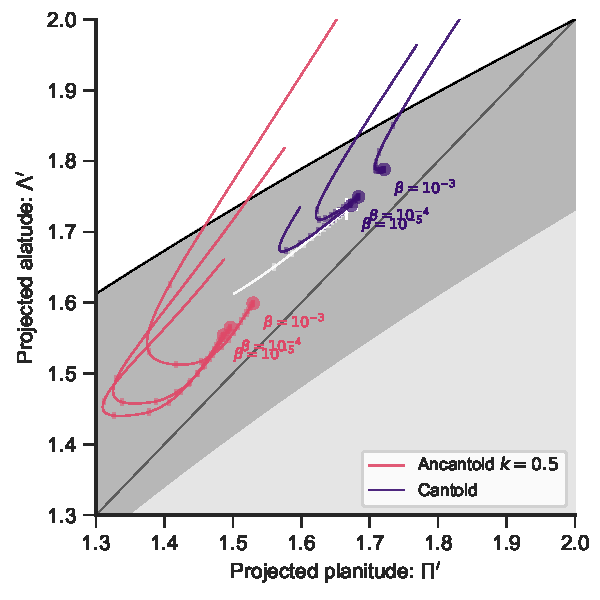
\includegraphics[width=\linewidth]{figs/ancantoid-R90-vs-Rc-lobeta-a}
  \caption[]{As Fig.~\ref{fig:thin-shell-R90-Rc}a but zoomed in to show
    the wilkinoid track (white) and the convergence of the cantoid
    tracks (purple) to the wilkinoid as \(\beta \to 0\).}
  \label{fig:convergence-cantoid-wilkinoid}
\end{figure}

The local density of tick marks gives an indication of how likely it
would be to observe each portion of the track, assuming an isotropic
distribution of viewing angles.  It can be seen that the ticks tend to
be concentrated towards the beginning of each track, near the
\(\abs{i} = 0\) point, so the hyperboloid-like portions of the tracks
would be observed for only a relatively narrow range of inclinations.
This concentration becomes more marked as \(\beta\) becomes smaller, which
helps to resolve the apparent paradox that the wilkinoid corresponds
to the \(\beta \to 0\) limit of the cantoids, and yet follows a
qualitatively different track.  The detailed behavior of the
small-\(\beta\) cantoid models is shown in
Figure~\ref{fig:convergence-cantoid-wilkinoid}, which zooms in on the
region around the wilkinoid track.  It can be seen that for
\(\beta < 0.001\) the cantoid tracks begin to develop a downward hook,
similar to the \(k = 0.5\) ancantoids discussed above.  For
\(\beta < 10^{-4}\) this begins to approach the wilkinoid track and the
high inclination, upward portion of the track becomes less and less
important as \(\beta\) decreases.




% \begin{figure*}
%   \centering
%   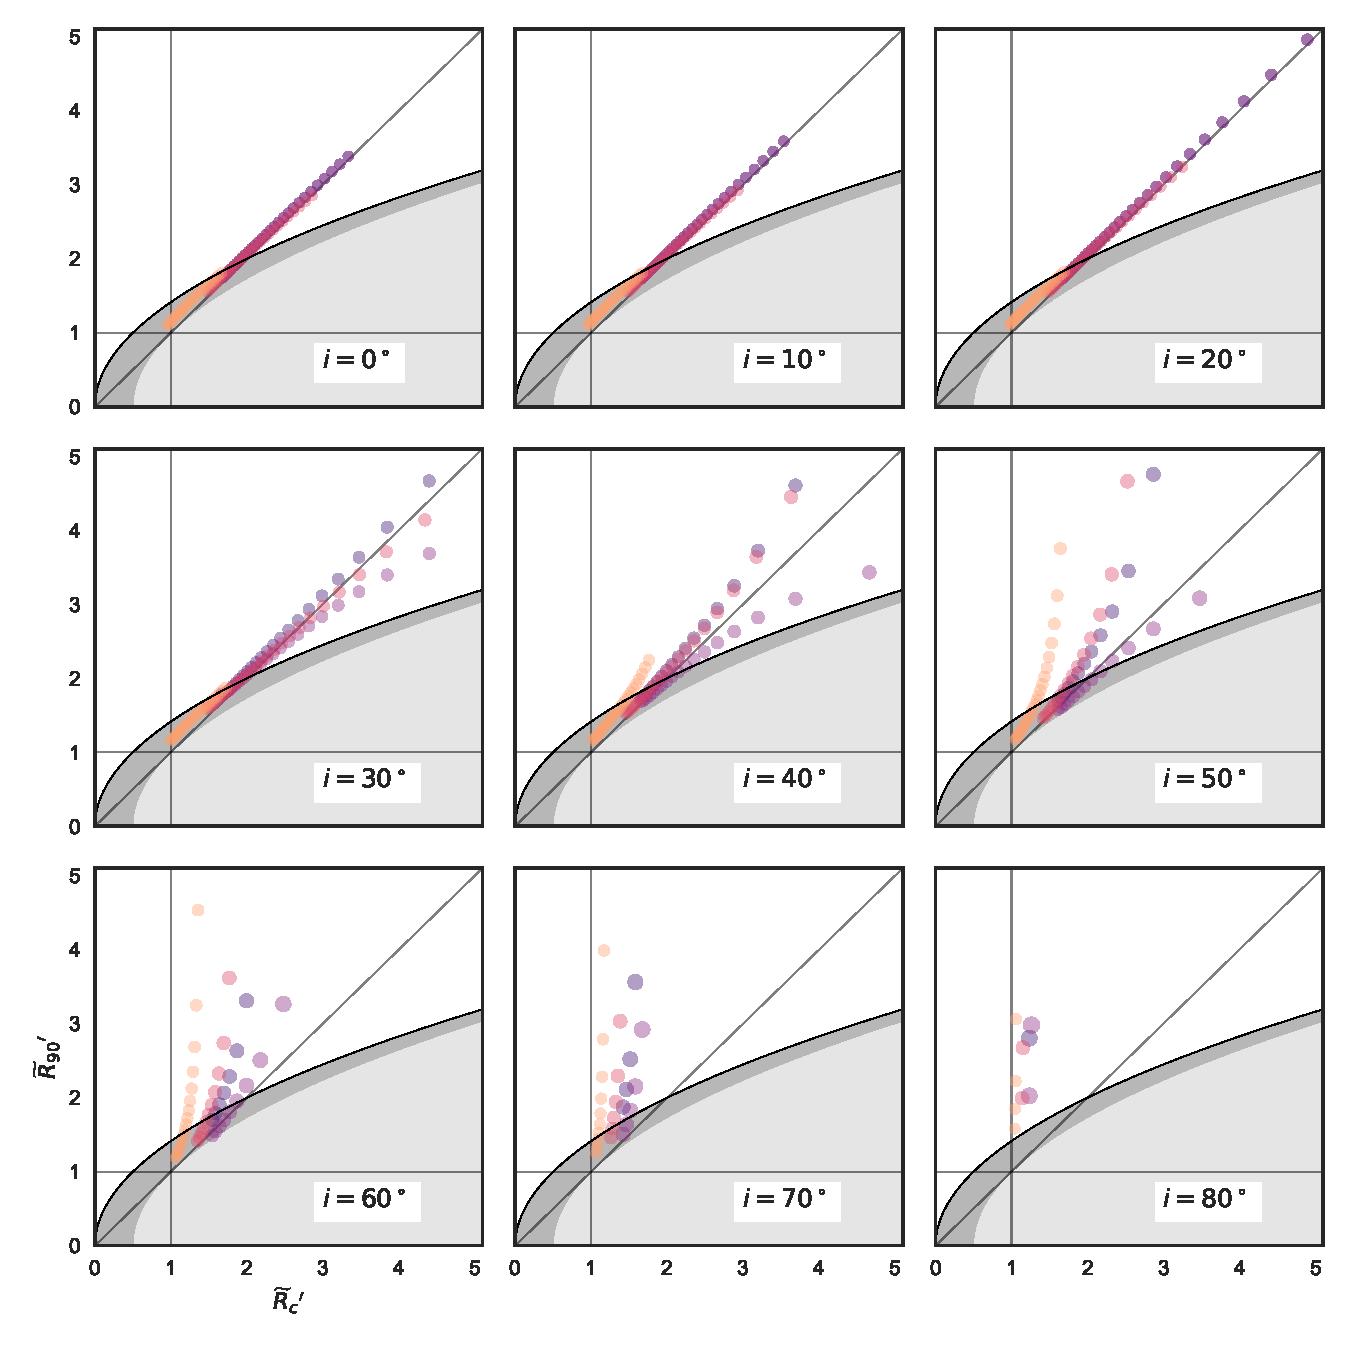
\includegraphics[width=0.8\textwidth]{figs/two-quadric-R90-Rc-snapshots}
%   \caption{Variation with inclination angle of radii diagnostics}
%   \label{fig:thin-shell-R90-Rc-snapshots}
% \end{figure*}


%%% Local Variables:
%%% mode: latex
%%% TeX-master: "quadrics-bowshock"
%%% End:
